

\tikzset{every picture/.style={line width=0.75pt}} %set default line width to 0.75pt        

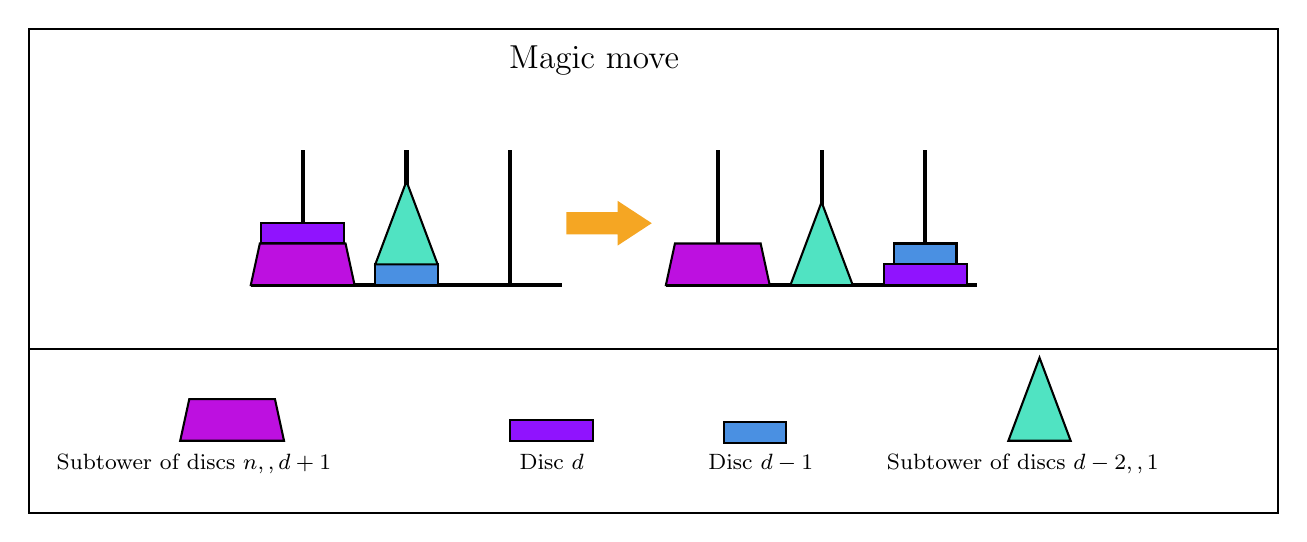
\begin{tikzpicture}[x=0.75pt,y=0.75pt,yscale=-1,xscale=1]
%uncomment if require: \path (0,365); %set diagram left start at 0, and has height of 365

%Straight Lines [id:da2433527856456119] 
\draw [line width=1.5]    (237,150) -- (237,85) ;
%Straight Lines [id:da12467546510005323] 
\draw [line width=1.5]    (287,150) -- (287,85) ;
%Straight Lines [id:da6661133221943116] 
\draw [line width=1.5]    (187,150) -- (187,85) ;
%Straight Lines [id:da876507202654921] 
\draw [line width=1.5]    (162,150) -- (312,150) ;
%Shape: Rectangle [id:dp9581710992755996] 
\draw  [fill={rgb, 255:red, 144; green, 19; blue, 254 }  ,fill opacity=1 ] (166.8,120) -- (206.8,120) -- (206.8,130) -- (166.8,130) -- cycle ;
%Shape: Rectangle [id:dp8402863453184108] 
\draw  [fill={rgb, 255:red, 74; green, 144; blue, 226 }  ,fill opacity=1 ] (222,140) -- (252,140) -- (252,150) -- (222,150) -- cycle ;
%Shape: Triangle [id:dp8282959416329734] 
\draw  [fill={rgb, 255:red, 80; green, 227; blue, 194 }  ,fill opacity=1 ] (237,100) -- (252,140) -- (222,140) -- cycle ;
%Shape: Trapezoid [id:dp17206160284989447] 
\draw  [fill={rgb, 255:red, 189; green, 16; blue, 224 }  ,fill opacity=1 ] (162,150) -- (166.35,130) -- (207.65,130) -- (212,150) -- cycle ;
%Straight Lines [id:da9363897255376088] 
\draw [line width=1.5]    (437,150) -- (437,85) ;
%Straight Lines [id:da5581881298896516] 
\draw [line width=1.5]    (487,150) -- (487,85) ;
%Straight Lines [id:da7500710046565593] 
\draw [line width=1.5]    (387,150) -- (387,85) ;
%Straight Lines [id:da03243354273668575] 
\draw [line width=1.5]    (362,150) -- (512,150) ;
%Shape: Rectangle [id:dp9137554325328925] 
\draw  [fill={rgb, 255:red, 144; green, 19; blue, 254 }  ,fill opacity=1 ] (467,140) -- (507,140) -- (507,150) -- (467,150) -- cycle ;
%Shape: Rectangle [id:dp8797795775448956] 
\draw  [fill={rgb, 255:red, 74; green, 144; blue, 226 }  ,fill opacity=1 ] (472,130) -- (502,130) -- (502,140) -- (472,140) -- cycle ;
%Shape: Triangle [id:dp4235756866358773] 
\draw  [fill={rgb, 255:red, 80; green, 227; blue, 194 }  ,fill opacity=1 ] (437,110) -- (452,150) -- (422,150) -- cycle ;
%Shape: Trapezoid [id:dp5348042276434657] 
\draw  [fill={rgb, 255:red, 189; green, 16; blue, 224 }  ,fill opacity=1 ] (362,150) -- (366.35,130) -- (407.65,130) -- (412,150) -- cycle ;
%Right Arrow [id:dp7411885527918458] 
\draw  [draw opacity=0][fill={rgb, 255:red, 245; green, 166; blue, 35 }  ,fill opacity=1 ] (314,114.81) -- (338.71,114.81) -- (338.71,109.41) -- (355.18,120.2) -- (338.71,131) -- (338.71,125.6) -- (314,125.6) -- cycle ;
%Shape: Trapezoid [id:dp5761586813750981] 
\draw  [fill={rgb, 255:red, 189; green, 16; blue, 224 }  ,fill opacity=1 ] (128,225) -- (132.35,205) -- (173.65,205) -- (178,225) -- cycle ;

%Shape: Rectangle [id:dp06928548817899349] 
\draw  [fill={rgb, 255:red, 144; green, 19; blue, 254 }  ,fill opacity=1 ] (287,215) -- (327,215) -- (327,225) -- (287,225) -- cycle ;

%Shape: Rectangle [id:dp9354576026846262] 
\draw  [fill={rgb, 255:red, 74; green, 144; blue, 226 }  ,fill opacity=1 ] (390,216) -- (420,216) -- (420,226) -- (390,226) -- cycle ;

%Shape: Triangle [id:dp5043879724591793] 
\draw  [fill={rgb, 255:red, 80; green, 227; blue, 194 }  ,fill opacity=1 ] (542,185) -- (557,225) -- (527,225) -- cycle ;

%Shape: Rectangle [id:dp8162339810622232] 
\draw   (55,26.5) -- (656.82,26.5) -- (656.82,259.95) -- (55,259.95) -- cycle ;
%Straight Lines [id:da9346086239123819] 
\draw    (55,180.95) -- (656.82,180.95) ;

% Text Node
\draw (285,33) node [anchor=north west][inner sep=0.75pt]  [font=\large] [align=left] {Magic move};
% Text Node
\draw (67,230) node [anchor=north west][inner sep=0.75pt]  [font=\footnotesize] [align=left] {Subtower of discs $\displaystyle n,\dotsc ,d+1$};
% Text Node
\draw (290,230) node [anchor=north west][inner sep=0.75pt]  [font=\footnotesize] [align=left] {Disc $\displaystyle d$};
% Text Node
\draw (381,230) node [anchor=north west][inner sep=0.75pt]  [font=\footnotesize] [align=left] {Disc $\displaystyle d-1$};
% Text Node
\draw (467,230) node [anchor=north west][inner sep=0.75pt]  [font=\footnotesize] [align=left] {Subtower of discs $\displaystyle d-2,\dotsc ,1$};


\end{tikzpicture}